\documentclass{article}

\usepackage[most]{tcolorbox}
\usepackage{physics}
\usepackage{graphicx}
\usepackage{float}
\usepackage{amsmath}
\usepackage{amssymb}


\usepackage[utf8]{inputenc}
\usepackage[a4paper, margin=1in]{geometry} % Controla los márgenes
\usepackage{titling}

\title{Agujeros Negros Cuánticos}
\author{Manuel Garcia.}
\date{\today}

\renewcommand{\maketitlehooka}{%
  \centering
  \vspace*{0.05cm} % Espacio vertical antes del título
}

\renewcommand{\maketitlehookd}{%
  \vspace*{2cm} % Espacio vertical después de la fecha
}

\newcommand{\caja}[3]{%
  \begin{tcolorbox}[colback=#1!5!white,colframe=#1!25!black,title=#2]
    #3
  \end{tcolorbox}%
}

\begin{document}
\maketitle

\section{Campos sobre variedades curvas }
Para un oscilador armónico: 
\begin{gather*}
  \frac{L }{2} \displaystyle\sum_{n=1 }^{ \infty} \left[\frac{1}{2}\rho \dot A _n^2 + \frac{1}{2} \rho \omega_n^2 A^2_n \right] \\
  \hat H \ket{n } = E_n \ket{n } \\
  E = \displaystyle\sum_{i=1 }^{\infty} (n_i + \frac{1}{2}) \hbar  \omega
\end{gather*}

\textbf{Coordenadas de Kruskal}
\begin{figure}[H]
  \begin{center}
    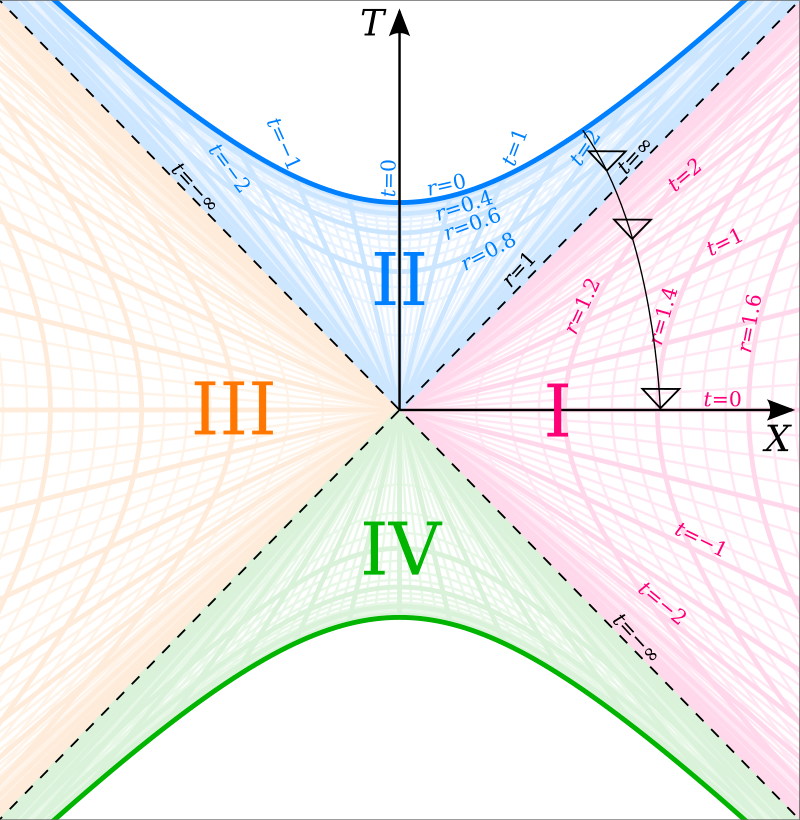
\includegraphics[width=0.3\textwidth]{kruskal.png}
  \end{center}
\end{figure}
\begin{gather*}
  (\Box - m^2 )  \phi = 0 \\
  \Box = \frac{\partial  }{\partial t } \left[(-\eta)^{\frac{1}{2}}\eta ^ {00 } \frac{\partial  }{\partial t }\right] + \frac{\partial  }{\partial x^a  } \left[(-\eta) ^ {\frac{1}{2}}\eta ^{ab } \frac{\partial  }{\partial x^b}\right] \qquad \qquad \eta = det(\eta _{\mu\nu} )
\end{gather*}

\hfill


\hfill

De forma general 

\begin{gather*}
  \Box =
    (-g) ^ {-\frac{1}{2}}\frac{\partial  }{\partial t } \left[(-g) ^ {\frac{1}{2}}g ^ {00 } \frac{\partial  }{\partial t }\right] 
  + (-g) ^ {-\frac{1}{2}}\frac{\partial  }{\partial x^a} \left[(-g) ^ {\frac{1}{2}} g ^{ab } \frac{\partial  }{\partial x^b}\right] 
\end{gather*}



\end{document}
